Given is the periodic signal curve $s(t)$, so that ${s_g}_0=\sqrt{3}/2$ and $\hat{s}_0=1$ applies

\begin{figure}[H]
	\centering
	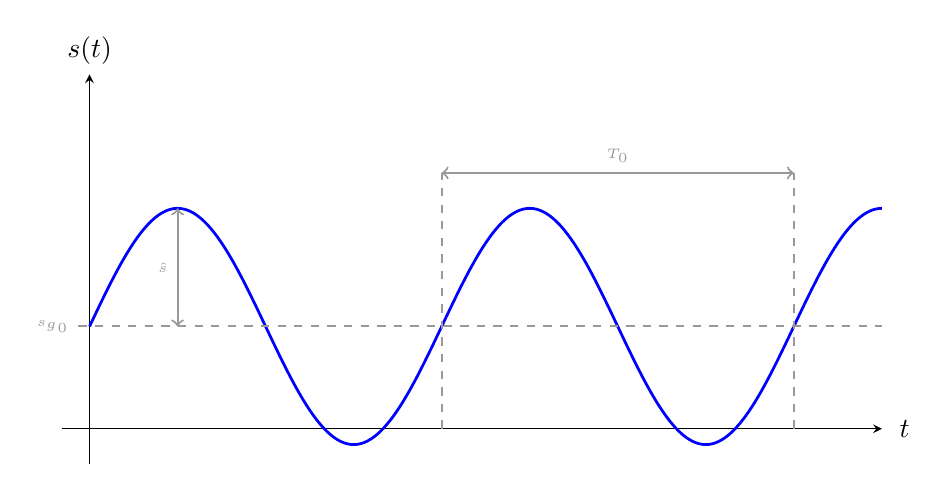
\begin{tikzpicture}
		\pgfplotsset{
			every axis plot/.append style={line width=1pt, mark=none}
		}
		\begin{axis}[
			clip=false,
			axis lines=middle,
			xmin=-0.5, xmax=4.5*pi,
			xlabel={$t$},
			xmajorticks=false,
			ymajorticks=false,
			ymin=-0.3,ymax=3,
			y=1.5cm,
			ylabel={$s(t)$},
			width=12cm,
			x label style={at={(current axis.right of origin)},	anchor=east, right=1mm},
			y label style={at={(current axis.above origin)}, anchor=south },
		]
			\addplot [samples=500, color=blue, domain=0:4.5*pi] {1*sin(deg(x))+sqrt(3)/2};
			\draw[color=gray!80, line width=0.75pt, dashed] (-0.2, {sqrt(3)/2}) -- (4.5*pi, {sqrt(3)/2});
			\draw[color=gray!80] node[left] at (-0.2,{sqrt(3)/2}) {\tiny ${s_g}_0$};
			
			\draw[color=gray!80, line width=0.75pt, dashed] (2*pi, 0) -- (2*pi, {sqrt(3)/2+1.3});
			\draw[color=gray!80, line width=0.75pt, dashed] (4*pi, 0) -- (4*pi, {sqrt(3)/2+1.3});
			\draw[<->, color=gray!80, line width=0.75pt] (2*pi, {sqrt(3)/2+1.3}) -- (4*pi, {sqrt(3)/2+1.3}) node[midway, above] {\tiny $T_0$};
			{1*sin(deg(x))+sqrt(3)/2}
			
			\draw[<->, color=gray!80, line width=0.75pt] (pi/2, {sqrt(3)/2}) -- (pi/2, {1*sin(deg(pi/2))+sqrt(3)/2}) node[midway, left] {\tiny $\hat{s}$};
			
		\end{axis}
	\end{tikzpicture}
	\caption{\label{fig:417}Characteristics of a periodic signal $s(t)$ with offset}
\end{figure}

The following applies for all calculations:
\begin{equation*}
	s(t) =\hat{s}\cdot\sin\left({\omega_0t}\right)+ s_{g_0}=
	1\cdot\sin\left({\omega_0t}\right)+\frac{\sqrt{3}}{2}
\end{equation*}

\begin{enumerate}
	\item Mean(Gleichwert) of the sinusoidal alternating variable
	From a mathematical point of view, the offset results in areas of different sizes when integrating over the period duration $T_0$ between the signal and the time axis.
	
	\begin{figure}[H]
		\centering
		\begin{tikzpicture}[line cap=rect]
			\pgfplotsset{
				every axis plot/.append style={line width=1pt, mark=none}
			}
			\begin{axis}[
				clip=false,
				axis lines=middle,
				xmin=-0.5, xmax=4.5*pi,
				xlabel={$t$},
				xmajorticks=false,
				ymajorticks=false,
				ymin=-0.3,ymax=3,
				y=1.5cm,
				ylabel={$s(t)$},
				width=12cm,
				x label style={at={(current axis.right of origin)},	anchor=east, right=1mm},
				y label style={at={(current axis.above origin)}, anchor=south },
			]
				\addplot [name path=positive, samples=500, color=green, domain=2*pi:4*pi, restrict y to domain=0:5] {sin(deg(x))+sqrt(3)/2};
				\addplot [name path=negative, samples=500, color=red, domain=2*pi:4*pi, restrict y to domain=-1:0] {sin(deg(x))+sqrt(3)/2};
				
				\path[name path=axis] (axis cs:0,0) -- (axis cs:4.5*pi,0);
				\addplot [fill=red, fill opacity=0.05]
					fill between[of=negative and axis, soft clip={domain=2*pi:4*pi}];
					
					
				\addplot [fill=green, fill opacity=0.05]
					fill between[of=positive and axis, soft clip={domain=2*pi:4*pi}];
					
				\addplot [samples=500, color=blue, domain=0:2*pi] {sin(deg(x))+sqrt(3)/2};
				\addplot [samples=500, color=blue, domain=4*pi:4.5*pi] {sin(deg(x))+sqrt(3)/2};
				
				
				\draw[color=gray!80, line width=0.75pt, dashed] (-0.2, {sqrt(3)/2}) -- (4.5*pi, {sqrt(3)/2});
				\draw[color=gray!80] node[left] at (-0.2,{sqrt(3)/2}) {\tiny ${s_g}_0$};
				\draw[color=gray!80, line width=0.75pt, dashed] (2*pi, 0) -- (2*pi, {sqrt(3)/2+1.3});
				\draw[color=gray!80, line width=0.75pt, dashed] (4*pi, 0) -- (4*pi, {sqrt(3)/2+1.3});
				\draw[<->, color=gray!80, line width=0.75pt] (2*pi, {sqrt(3)/2+1.3}) -- (4*pi, {sqrt(3)/2+1.3}) node[midway, above] {\tiny $T_0$};
				{1*sin(deg(x))+sqrt(3)/2}
				
				\draw[<->, color=gray!80, line width=0.75pt] (pi/2, {sqrt(3)/2}) -- (pi/2, {1*sin(deg(pi/2))+sqrt(3)/2}) node[midway, left] {\tiny $\hat{s}$};
				
			\end{axis}
		\end{tikzpicture}
		\captionsetup{format=hang,justification=raggedright}
		\caption{\label{fig:417a}Signal $s(t)$ with integration areas\\(green - positive component; - red negative component)}
	\end{figure}
	

	\begin{equation*}
		\overline{s} = \frac{1}{T_0}\int_{t_0}^{t_0+T_0}s(t)\D{t}
	\end{equation*}
	{
		\setlength{\abovedisplayskip}{6pt}
		\setlength{\belowdisplayskip}{12pt}
		\begin{flalign*}
			\overline{s} &=\frac{1}{T_0}\int_{0}^{T_0}{s(t)}\D{t}
			= \frac{1}{T_0}\int_{0}^{T_0}\sin({\omega_0t})+\frac{\sqrt{3}}{2}\D{t} & \\
			& = \frac{1}{T_0}\int_{0}^{T_0}\sin({\omega_0t})\D{t} + \int_{0}^{T_0}\frac{\sqrt{3}}{2}\D{t} & \\
			& = \frac{1}{T_0} \left(\frac{1}{\omega_0}\Big[-\cos(\omega_0t)\Big]_0^{T_0} + \left[\frac{\sqrt{3}}{2}t\right]_0^{T_0} \right) & \\
			& = \frac{1}{\cancel{T_0}} \frac{1}{\frac{2\pi}{\cancel{T_0}}}\left[-\cos\left(\frac{2\pi}{\cancel{T_0}}\cancel{T_0}\right)-\big(-\cos(0)\big)\right]
			+ \frac{1}{\cancel{T_0}} \left[\frac{\sqrt{3}}{2}\cancel{T_0}-\frac{\sqrt{3}}{2}\cdot0\right] & \\
			& = \frac{1}{2\pi}\left[-\cos\left(2\pi\right)+\cos(0)\right]
			+ \frac{\sqrt{3}}{2} & \\
			& = \frac{\sqrt{3}}{2} & 
		\end{flalign*}
	}
	
	\item Average absolute value <AAV>(Gleichrichtwert) of the sinusoidal alternating variable
	\begin{equation*}
		\overline{\abs{s}} = \frac{1}{T_0}\int_{t_0}^{t_0+T_0}\abs{s(t)}\D{t}
	\end{equation*}	
	The following rectified signal results from Figure ~\ref{fig:417a} after rectification due to the asymmetrical distribution around the time axis
	
	\begin{figure}[H]
		\centering
		\begin{tikzpicture}[line cap=rect]
			\pgfplotsset{
				every axis plot/.append style={line width=1pt, mark=none}
			}
			\begin{axis}[
				clip=false,
				axis lines=middle,
				xmin=-0.5, xmax=4.5*pi,
				xlabel={$t$},
				xmajorticks=false,
				ymajorticks=false,
				ymin=-0.3,ymax=3,
				y=1.5cm,
				ylabel={$s(t)$},
				width=12cm,
				x label style={at={(current axis.right of origin)},	anchor=east, right=1mm},
				y label style={at={(current axis.above origin)}, anchor=south },
			]
				\addplot [name path=f1, samples=500, color=blue, domain=0:4.5*pi, restrict y to domain=0:5] {sin(deg(x))+sqrt(3)/2};
				\addplot [samples=500, color=blue!60, domain=0:4.5*pi, restrict y to domain=-1:0, dashed] {sin(deg(x))+sqrt(3)/2};
				\addplot [name path=f2, samples=500, color=blue, domain=0:4.5*pi, restrict y to domain=0:1] {sin(-deg(x))+sqrt(3)/2*-1};
			
				\path[name path=axis] (axis cs:0,0) -- (axis cs:4.5*pi,0);
				\addplot [fill=blue, fill opacity=0.05]
					fill between[of=f1 and axis, soft clip={domain=2*pi:4*pi}];
					
				\addplot [fill=blue, fill opacity=0.05]
					fill between[of=f2 and axis, soft clip={domain=2*pi:4*pi}];
				
				\draw[color=gray!80, line width=0.75pt, dashed] (-0.2, {sqrt(3)/2}) -- (4.5*pi, {sqrt(3)/2});
				\draw[color=gray!80] node[left] at (-0.2,{sqrt(3)/2}) {\tiny ${s_g}_0$};
				
				\draw[color=gray!80, line width=0.75pt, dashed] (2*pi, 0) -- (2*pi, {sqrt(3)/2+1.3});
				\draw[color=gray!80, line width=0.75pt, dashed] (4*pi, 0) -- (4*pi, {sqrt(3)/2+1.3});
				\draw[<->, color=gray!80, line width=0.75pt] (2*pi, {sqrt(3)/2+1.3}) -- (4*pi, {sqrt(3)/2+1.3}) node[midway, above] {\tiny $T_0$};
				
				\draw[<->, color=gray!80, line width=0.75pt] (pi/2, {sqrt(3)/2}) -- (pi/2, {1*sin(deg(pi/2))+sqrt(3)/2}) node[midway, left] {\tiny $\hat{s}$};
			\end{axis}
		\end{tikzpicture}
		\caption{\label{fig:417b}Rectified signal $s(t)$}
	\end{figure}
	A closer look at Figure ~\ref{fig:417b} reveals two integration areas in the $T_0$ range. These become clear when the period is shifted to the intersection points of the rectified signal components (zero crossing).	
	\begin{figure}[H]
		\centering
		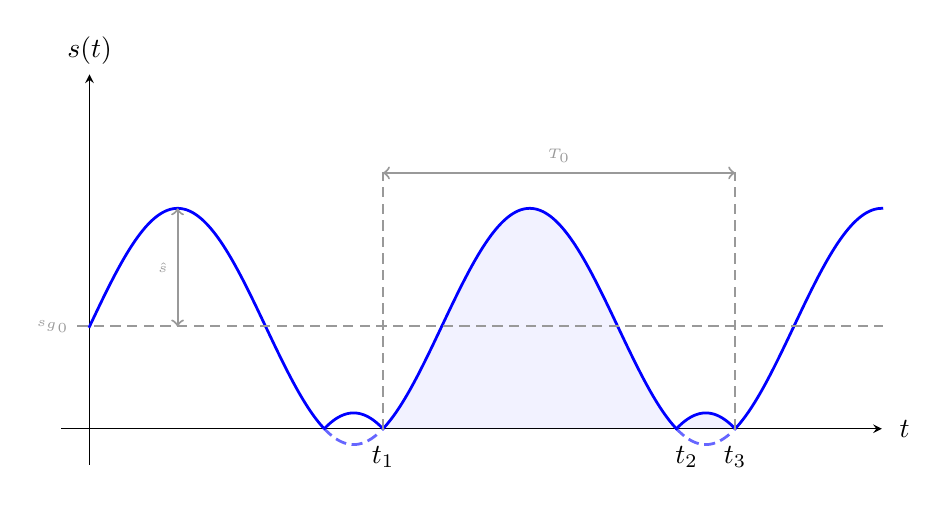
\begin{tikzpicture}[line cap=rect]
			\pgfplotsset{
				every axis plot/.append style={line width=1pt, mark=none}
			}
			\begin{axis}[
				clip=false,
				axis lines=middle,
				xmin=-0.5, xmax=4.5*pi,
				xlabel={$t$},
				xmajorticks=false,
				ymajorticks=false,
				ymin=-0.3,ymax=3,
				y=1.5cm,
				ylabel={$s(t)$},
				width=12cm,
				x label style={at={(current axis.right of origin)},	anchor=east, right=1mm},
				y label style={at={(current axis.above origin)}, anchor=south },
			]
			
				\addplot [samples=500, color=blue, domain=0:{2*pi - rad(asin(sqrt(3)/2))}, restrict y to domain=0:5] {sin(deg(x))+sqrt(3)/2};
				\addplot [samples=500, color=blue, domain={4*pi - rad(asin(sqrt(3)/2))}:{4.5*pi}, restrict y to domain=0:5] {sin(deg(x))+sqrt(3)/2};
				\addplot [samples=500, color=blue!60, domain=0:4.5*pi, restrict y to domain=-1:0, dashed] {sin(deg(x))+sqrt(3)/2};
				\addplot [samples=500, color=blue, domain=0:{2*pi - rad(asin(sqrt(3)/2))}, restrict y to domain=0:1] {sin(-deg(x))+sqrt(3)/2*-1};
				\addplot [samples=500, fill=blue, fill opacity=0.05, color=blue, domain={2*pi - rad(asin(sqrt(3)/2))}:{4*pi - rad(asin(sqrt(3)/2))}, restrict y to domain=0:5] {sin(deg(x))+sqrt(3)/2};
				
				\addplot [samples=500, fill=blue, fill opacity=0.05, draw=blue, domain={2*pi - rad(asin(sqrt(3)/2))}:{4*pi - rad(asin(sqrt(3)/2))}, restrict y to domain=0:1] {sin(-deg(x))+sqrt(3)/2*-1};
				
				\draw[color=gray!80, line width=0.75pt, dashed] (-0.2, {sqrt(3)/2}) -- (4.5*pi, {sqrt(3)/2});
				\draw[color=gray!80] node[left] at (-0.2,{sqrt(3)/2}) {\tiny ${s_g}_0$};
				
				\draw[color=gray!80, line width=0.75pt, dashed]
					({2*pi - rad(asin(sqrt(3)/2))}, 0) -- ({2*pi - rad(asin(sqrt(3)/2))}, {sqrt(3)/2+1.3});
				\draw[color=gray!80, line width=0.75pt, dashed]
					({4*pi - rad(asin(sqrt(3)/2))}, 0) -- ({4*pi - rad(asin(sqrt(3)/2))}, {sqrt(3)/2+1.3});
				\draw[<->, color=gray!80, line width=0.75pt]
					({2*pi - rad(asin(sqrt(3)/2))}, {sqrt(3)/2+1.3}) -- ({4*pi - rad(asin(sqrt(3)/2))}, {sqrt(3)/2+1.3}) node[midway, above] {\tiny $T_0$};
				
				\draw[<->, color=gray!80, line width=0.75pt]
					(pi/2, {sqrt(3)/2}) -- (pi/2, {sin(deg(pi/2))+sqrt(3)/2}) node[midway, left] {\tiny $\hat{s}$};
				
				\node at ({2*pi - rad(asin(sqrt(3)/2))}, 0)[below=3pt] {$t_1$};
				\node at ({4*pi - rad(asin(sqrt(3)/2)) - sqrt(3)/2)}, 0)[below=3pt] {$t_2$};
				\node at ({4*pi - rad(asin(sqrt(3)/2))}, 0)[below=3pt] {$t_3$};
					
			\end{axis}
		\end{tikzpicture}
		\captionsetup{justification=centering}
		\caption{\label{fig:417c}Rectified signal $s(t)$\\with shifted period duration in the zero crossings}
	\end{figure}
	
	\underline{Zero point calculation:}\\
	\begin{tabularx}{\linewidth}{rlll}
		$s(t)$ & $=$ & $0$ & \\[1.5ex]
		$\sin(\omega_0\cdot{t}) + \dfrac{\sqrt{3}}{2}$ & $=$ & $0$ & $\quad \left|\;- \dfrac{\sqrt{3}}{2}\right. $ \\[1.5ex]
		$\sin(\omega_0\cdot{t})$ & $=$ & $-\dfrac{\sqrt{3}}{2}$    & $\quad \left|\; \Rightarrow \omega_0\cdot{t_2} = \dfrac{4\pi}{3}\;\right.$ \\[1.5ex]
		&&& \phantom{$\quad |\;\Rightarrow$}$\omega_0\cdot{t_3} = \dfrac{5\pi}{3}$  \\[1.5ex]
		&&& \phantom{$\quad |\;\Rightarrow$}(from unit circle) \\[1.5ex]
	\end{tabularx}
	
	\underline{Calculation of the integral:}\\
	
	
	
	
%	{
%		\setlength{\abovedisplayskip}{6pt}
%		\setlength{\belowdisplayskip}{12pt}
%		\begin{flalign*}
%			\overline{s} &=\frac{1}{T_0}\int_{0}^{T_0}{s(t)}\D{t}
%			= \frac{1}{T_0}\int_{0}^{T_0}\sin({\omega_0t})+\frac{\sqrt{3}}{2}\D{t} & \\
%			& = \frac{1}{T_0}\int_{0}^{T_0}\sin({\omega_0t})\D{t} + \int_{0}^{T_0}\frac{\sqrt{3}}{2}\D{t} & \\
%			& = \frac{1}{T_0} \left(\frac{1}{\omega_0}\Big[-\cos(\omega_0t)\Big]_0^{T_0} + \left[\frac{\sqrt{3}}{2}t\right]_0^{T_0} \right) & \\
%			& = \frac{1}{\cancel{T_0}} \frac{1}{\frac{2\pi}{\cancel{T_0}}}\left[-\cos\left(\frac{2\pi}{\cancel{T_0}}\cancel{T_0}\right)-\big(-\cos(0)\big)\right]
%			+ \frac{1}{\cancel{T_0}} \left[\frac{\sqrt{3}}{2}\cancel{T_0}-\frac{\sqrt{3}}{2}\cdot0\right] & \\
%			& = \frac{1}{2\pi}\left[-\cos\left(2\pi\right)+\cos(0)\right]
%			+ \frac{\sqrt{3}}{2} & \\
%			& = \frac{\sqrt{3}}{2} & 
%		\end{flalign*}
%	}
%	
%	{
%		\setlength{\abovedisplayskip}{6pt}
%		\setlength{\belowdisplayskip}{12pt}
%		\begin{flalign*}
%			\overline{\abs{s}} &= \frac{1}{T_0}\cdot2\int_{0}^{\frac{T_0}{2}}{s(t)}\D{t}
%			=\frac{1}{T_0}\cdot2\int_{0}^{\frac{T_0}{2}}\hat{s}\cdot\sin\left(\omega_0\cdot{t}\right)\D{t}
%			=\frac{2\hat{s}}{T_0}\int_{0}^{\frac{T_0}{2}}\sin\left(\omega_0\cdot{t}\right)\D{t} & \\
%			& = \frac{2\hat{s}}{T_0}\cdot\left[\frac{-\cos\left(\omega_0\cdot{t}\right)}{\omega_0}\right]_0^{\frac{T_0}{2}}
%			= \frac{\cancel{2}\hat{s}}{\bcancel{T_0}}\cdot\left[\frac{-\cos\left(\frac{2\pi}{T_0}t\right)}{\frac{\cancel{2}\pi}{\bcancel{T_0}}}\right]_0^{\frac{T_0}{2}} & \\
%			& = \frac{\hat{s}}{\pi}\left(-\cos\left(\frac{\cancel{2}\pi}{\bcancel{T_0}}\cdot\frac{\bcancel{T_0}}{\cancel{2}}\right)+\cos\left(\frac{2\pi}{T_0}\cdot0\right)\right)
%			= \frac{\hat{s}}{\pi} \left(-\cos\left(\pi\right)+\cos(0)\right) & \\
%			& = \frac{2\hat{s}}{\pi} \approx \num{0,636}\overline{6}\;\hat{s}
%		\end{flalign*}
%	}
	
	\item Description and visualization in Matlab
	\lstinputlisting[language=Matlab]{./assets/Lab1_417.m}
	{
		\setlength{\fboxsep}{0pt}%  
		\colorbox{backcolor}{\includegraphics[width=\linewidth, keepaspectratio]{./assets/417.png}}
	}	
\end{enumerate}
\clearpage